\section*{WOLF}
WOLF is a framework that is composed of tasks of machine learning from preprocessing of data to selecting the best model for that data. It allows a user to control each of these steps of the machine learning pipeline however they desire for a supervised classification problem. The models WOLF supports are:
\begin{itemize}
\item AdaBoost
\item Bernoulli Naive Bayes
\item Gaussian Naive Bayes
\item Decision Tree (DT)
\item Logistic Regression (LR)
\item Random Forest (RF)
\item C-Support Vector Machine(C-SVM)
\item Linear Support Vector Machine (Linear SVM)
\item Nu Support Vector Machine (Nu SVM)
\item Linear Discriminant Analysis (LDA)
\item Quadratic Discriminant Analysis (QDA)
\item Deep Neural Network (DNN)
\end{itemize}

WOLF splits each step of the ML pipeline into an individual task but they are usually dependent on previous tasks, e.g., all models are trained separately, but the metric calculation cannot be performed until the model training is complete. Each of these tasks are called ``transactions". The WOLF configuration file is a {\tt yaml} file that is fully customizable to choose which dataset to use, which transactions to run, and how to run these transactions. The transactions you could choose from and modify are pre-processing, splitting data, feature extraction, feature selection, model construction, metric evaluation, and model selection. A visual representation of the workflow can be seen in Figure \ref{fig:original WOLF workflow}.

\begin{figure}[H]
	\centering
	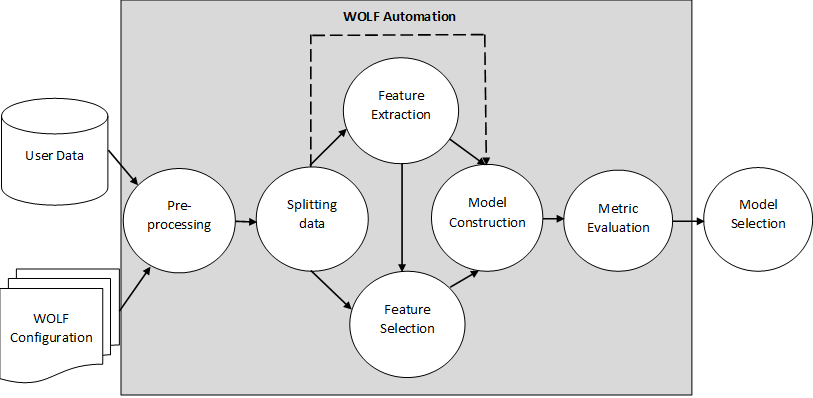
\includegraphics[scale=0.65]{original_arch}
	\caption{Original WOLF architecture \parencite{WOLFprojectreport}}
	\label{fig:original WOLF workflow}
\end{figure}

Not all of the transactions are mandatory. The dotted line signals that a user can skip feature extraction and/or feature selection if they want. A user also does not have do any pre-processing if their data is already in the correct format. All other transactions are required for WOLF to work though. Each transaction performs a vital step in the pipeline.
\begin{itemize}
	\item \textbf{Pre-Processing:} Performs any step that would be needed to make the dataset complete for WOLF. Some of these actions would include replacing any missing values with a user specified value or scaling numerical values from a provided ratio. An important step in pre-processing is to encode all categorical features and labels into a numerical value.
	\item \textbf{Splitting Data:} Splits the data into train and test files. There are two values the user provides: number of folds and number of repetitions. The number of times is the number of train and test files to create. This allows cross-validation to be performed. The repetitions value is the number of times to perform the split. The splits are performed on a randomized order of the dataset.
	\item \textbf{Feature Extraction:} Uses the train and test files as input and attempts to perform dimensionality reduction. This could lead to new features being created that combine multiple features in the dataset. (Optional)
	\item \textbf{Feature Selection:} This step selects features that are too noisy to be meaningful or will be redundant in the model and removes them. It then creates new train and test files with the selected features removed. (Optional)
	\item \textbf{Model Construction:} This is the transaction where most of the work is done. For each machine learning model type and each combination of hyper-parameters that are to be tested on, a model is trained on every train/test set combination. This will output the hyper-parameters used along with the predictions that were made from the model.
	\item \textbf{Model Evaluation:} After each model is trained, different metrics are calculated based on the true values and the predictions. These metrics can include accuracy, precision, area under the curve receiver operating characteristics (ROC-AUC), Matthew's correlation coefficient (MCC), F1-Score, and the capability for more. These are the metrics that will be used for choosing the best model.
	\item \textbf{Model Selection:} This transaction takes the model metrics as input and determines the be best model and hyper-parameter combination. All of the metrics are written to a results excel file and sorted by a chosen metric. In this file the best configuration is also given.
\end{itemize}

To keep track of the data as it flows through the pipeline, a non-relational database, MongoDB, is used. Every configuration and parameter is stored and an id value for the run is used to keep track of each WOLF configuration run. There are seven databases and each holds collections to store the values. These databases mainly follow the format of the transactions. The databases are Pre-Processing, Split Data, Files, Feature Extraction, Feature Selection, Algorithm, and Result. Each value that would be in a collection stored in the database can be seen in Figure \ref{fig:original WOLF database}.

\begin{figure}[H]
	\centering
	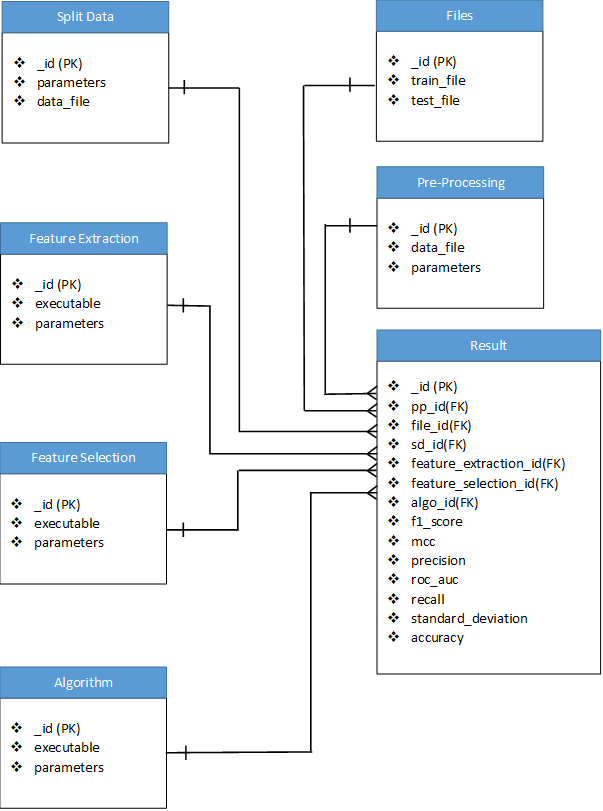
\includegraphics[scale=0.65]{original_db}
	\caption{Original WOLF MongoDB \parencite{WOLFprojectreport}}
	\label{fig:original WOLF database}
\end{figure}

Figure \ref{fig:wolf configuration} shows an example of a configuration file that uses all transactions and trains on three model types with varying hyper-parameter possibilities. There are two options when providing values for a hyper-parameter: ``single" and ``collection". If ``single" is chosen, one value is provided. If ``collection" is given, either ``list" or ``range" must chosen. A list is then provided and if ``list" then those are the values tested; if ``range" the values tested are all values between the first two numbers with a step size of the third.

\newpage
\begin{figure}[H]
	\centering
	\lstinputlisting[language=sh, basicstyle=\scriptsize]{configurations/wolf_yaml.sh}
	\caption{WOLF configuration file example}
	\label{fig:wolf configuration}
\end{figure}

\section*{Other Tools}
One popular tool that WOLF could be compared to and was an influence is Auto-WEKA \parencite{AutoWEKA}. It was developed in 2013 at the University of British Columbia. It is a downloadable tool that allows classification algorithms to be searched and for hyper-parameter optimization to be performed. It runs on 39 different classification algorithms. Tree-based Bayesian optimization is used to search through the hyper-parameter space as opposed to the grid search that WOLF provides.

Another important tool is Michelangelo \parencite{michelangelo}. It was created by Uber to, like WOLF, perform the machine learning workflow from beginning to end. The six steps in the workflow that Michelangelo follows are ``managing data, training models, evaluating models, deploying models, making predictions, and monitoring predictions''. It was made with the massive scale that Uber needs in mind and the goal of standardizing each step of the pipeline within the company. Thus, there is a shared feature store within the tool that teams can use for others to utilize in their work. Training the model returns many values on runs, including the best hyper-parameters, importance of features, and visualization of different metric scores. Deploying models is performed in a standardized way that meets the needs of the Uber model framework. Once deployed, predictions can be made on both data loaded in for testing and on real world data that can be monitored for performance. Michelangelo can be used both online and offline.